
\chapter{Hashtabellen}
Suchen in $\bigO{}(1)$ pro Query (d.h. $\bigO{}(N)$ zum Aufbau der Tabelle) \\

Trick wie bei bucket\_sort: i = hash(key)$\Rightarrow$ ganze Zahl $\in [0,M)$ \\
\hspace*{5mm} Unterschied zu quantize: hash(key) muss $\textbf{nicht}$ die Ordnung erhalten\\
\hspace*{10mm} $\Rightarrow$ mehr Freiheit bei der Auswahl von hash(key)\\
\hspace*{15mm} die selbe Hash-Funktion funktioniert für viele verschiedene Wahrscheinlichkeitsverteilun- \\
\hspace*{15mm} gen der keys.\\

Wertebereich von hash(): U $\widehat{=}$ \glqq Universum\grqq des Schlüssels \\
\hspace*{5mm} z.B. wenn key ein String der Länge 9, 60 erlaubte Zeichen \\
\[ |U| = 60^9 \approx 10^{16}\]
dagegen: $M \in \bigO{}(N) << |U|$ $\Rightarrow$ Viele Schlüssel werden durch hash(key) auf den gleichen Wert\\
\hspace*{15mm} abgebildet $\widehat{=}$ \textbf{Kollision}\\
gute Hashfunktion: Kollision für alle Schlüssel gleich wahrscheinlich \\
\hspace*{15mm} ($\widehat{=}$ bucket\_sort: alle Buckets sind gleich voll) \\

Beispiel: Monatsnummern als Schlüssel \verb|"Januar", "Februar", ..., "Dezember"| \\
hash(key) $\Rightarrow$ key[0] Anfangsbuchstabe: \\

\hspace*{10mm} \textcolor{red}{J} \hspace*{5mm}  F \hspace*{5mm}  \textcolor{blue}{M} \hspace*{5mm}  \textcolor{green}{A} \hspace*{5mm}  \textcolor{blue}{M} \hspace*{5mm}  \textcolor{red}{J} \hspace*{5mm}  \textcolor{red}{J} \hspace*{5mm}  \textcolor{green}{A} \hspace*{5mm}
 S \hspace*{5mm}  O \hspace*{5mm}  N \hspace*{5mm}  D \hspace*{10mm} viele Kollisionen \\

klassisch (Papierformulare) : hash(key)$\Rightarrow$ key[0:3] erste 3 Buchstaben\\
\hspace*{5mm} Jan, Feb, ... \hspace*{2.3cm} keine Kollision, aber M sehr groß ($60^3 = 216000 >> N$) \\

perfekte Hashfunktion: hash(key) $\Rightarrow$ [0,11] \hspace*{5mm} [1,12] \\

\section{Bewährte Hashfunktionen}
Idee: Interpretiere jeden Schlüssel als Bytefolge\\

\textbf{Bernstein:}
\begin{minted}{python}
def b_hash(u):          #u: Array of Bytes
    h = 0
    for i in u:
        h = 33*h + i    # 33 wurde experimentell bestimmt fuer wenig Kollision
    return h
\end{minted}
$h \in [0, \cdots, 2^{32} -1]$ int32 \\
$h \in [0, \cdots, 2^{64} -1]$ int64 \\


\textbf{modifizierte Bernstein:}
\begin{minted}{python}
def mb_hash(u):         #u: Array of Bytes
    h = 0
    for i in u:
        h = 33*h^i      # ^: bitweise XOR
    return h
\end{minted}

\textbf{shift-Add-XOR:}
\begin{minted}{python}
def sax_hash(u):
    h = 0
    for i in u:
        h^= (h << 5) + (h >> 2) + i
    return h
\end{minted}

\textbf{Fowler $|$ Noll $|$ Vo:}
\begin{minted}{python}
def FNV_hash(u):
    h = 2166136261
    for i in u:
        h = (16777619 * h)^i
    return h
\end{minted}
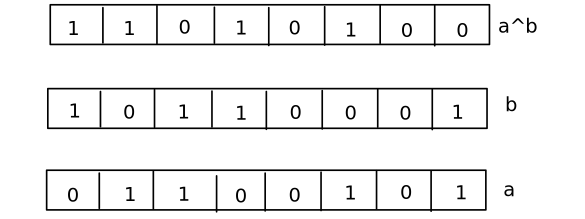
\includegraphics[width=7cm,height=3cm,keepaspectratio]{./Pictures/abArrays.png}

\section{Prinzip der Hashtabelle}
\begin{itemize}
    \item intern: Array der Länge M (dynamisches Array: vergrößere M falls N zu groß wird $\Rightarrow$ später)
    \item speichere Schlüssel key beim Index i =$\underbrace{\text{ hash(key)}}_{0...(2^{32}-1)} \% \underbrace{M}_{>> \bigO{}(N)} \in [0, M-1]$
    \item mache etwas trickreiches bei Kollision
    \begin{itemize}
        \item lineare Verkettung \hspace*{5mm} \glqq offenes Hashing\grqq \glqq geschlossene Adressierung\grqq
        \item offene Adressierung
        \item doppeltes Hashing
    \end{itemize}
\end{itemize}

\section{Hashtabelle mit linearer Verkettung}
\begin{itemize}
    \item wie bei bucket\_sort: für jeden Index hat man ein Array oder eine verkettete List, wo alle Schlüssel mit demselben Hash landen:
    \begin{minted}{python}
class HashNode:
    def __init__(self, key, value, next):
        self.key = key
        self.value = value
        self.next = next

class HashTabelle:
    def __init__(self):
        self.capacity = ...             # initiales M
        self.size = 0
        self.data = [None] * self_capacity

    def __setitem__(self, key, value):
        i = hash(key) % self.capacity   #bucket finden
        bucket = self.data[i]           #bucket finden
        while bucket is not None:
            if bucket.key == key:       #key war schon vorhanden
                bucket.value = value    # => value ersetzen
                return
            else:
                bucket = bucket.next     #durch verkettete Liste iterieren

        # wenn wir hier landen, war key noch nicht  vorhanden
        # => neues Element einfuegen

        new_node = HashNode(key, value, self.data[i])
        self.data[i] = new_node
        self.size += 1
        ... # hier eventuell die capacity vergroessern

    def __getitem__(self, key):
        i = hash(key) % self.capacity
        bucket = self.data[i]
        while bucket is not None:
            if bucket.key == key:
                return bucket.value
            bucket = bucket.next
        raise keyError(key)
    \end{minted}
\end{itemize}

\subsubsection*{Komplexität der Hash-Tabelle mit linearer Verkettung}
\begin{itemize}
    \item Ausrechnen des Hashs und finden des Buckets: $\bigO{}(1)$
    \item Schlüssel im Bucket suchen: ($N_i$: Länge Bucket i)
    \begin{itemize}
        \item vorhanden $\bigO{}\left(\frac{N_i}{2}\right)$
        \item nicht vorhanden $\bigO{}(N_i)$
    \end{itemize}
    \item mittlere Suchzeit für viele Aufrufe:
    \[ \mathbb{E}[t] = \sum_{i=0}^{M-1} p_i\bigO{}(N_i) \hspace*{3cm} M : \text{capacity} \]
    Annahme: gute Hash-Funktion $\Rightarrow$ Schlüssel gleichmäßig auf die Buckets verteilt\\ $\Rightarrow$ $p_i = \frac{1}{M}, \hspace*{1cm} N_i = \frac{N}{M}$
    \[ \mathbb{E}[t] = \sum_{i=0}^{M-1} \frac{1}{M} \bigO{} \left(\frac{N}{M}\right) = \bigO{} \left(\frac{N}{M^2}\right) \underbrace{\sum_{i=0}^{M-1} 1}_{=M} = \bigO{} \hspace*{-9mm} \underbrace{\left(\frac{N}{M}\right)}_{\text{Füllstand jedes Buckets}}\]
    \item Gesamtzeit soll $\bigO{}(1)$ sein:
    \[ \bigO{}(1)  \stackrel{!}{=} \bigO{}(1) + \underbrace{\bigO{}\left(\frac{N}{M}\right)}_{\bigO{}(1)} \Leftrightarrow M \in \bigO{}(N)\]
$\Rightarrow$ wenn Hashtabelle voll $\Rightarrow$ verdoppele Kapazität M \\
Trick: setze M als Primzahl $\Rightarrow$ keys werden gleichmäßiger verteilt bei hash(key)\%M
\[ M \in \{11, 23, 47, 97, 199, 409, 823, \cdots\}\]
z.B. häufig verwendet für C++ Klasse std::unordered\_map
\end{itemize}

\section{Hashtabellen mit offener Adressierung}
\begin{itemize}
    \item HT mit linearer Verkettung: pessimistisch $\widehat{=}$ es wird viele Kollisionen geben\\ \hspace*{3cm}$\Rightarrow$ jeder Index enthält von vornherein eine Liste von Keys
    \item HT mit offener Adressierung: optimistisch $\widehat{=}$ Kollisionen sind so selten, dass wir keine Liste für jeden Index brauchen\\ \hspace*{3cm}$\widehat{=}$ jeder Index enthält kein oder ein Element
    \item einfachste Variante: \textbf{sequentielles Sondieren}: wenn der gewünschte Index bereits belegt ist $\Rightarrow$ probiere den nächsten bis man einen freien Index findet \\
    Konsequenzen:
    \begin{itemize}
        \item capacity $>$ size notwendig, sonst Endlosschleife
        \item Entfernen von Elementen nicht mit naivem Vorgehen (Element auf None setzen) möglich\\
        \includegraphics[width=10cm,height=4cm,keepaspectratio]{./Pictures/naivesLöschen.png}\\
        statt dessen: gelöschte Elemente als \emph{gelöschte} markieren, damit die Suchkette bei Kollisionen nicht vorzeitig abbricht
    \end{itemize}
    Nachteil: Clusterbildung
    \begin{itemize}
        \item Bereiche, wo alle Indizes belegt sind
        \item Bereiche, wo alle Indizes frei sind\\
        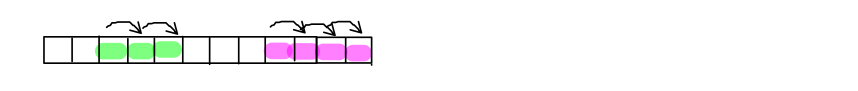
\includegraphics[width=10cm,height=3cm,keepaspectratio]{./Pictures/buntesArray.png}\\
        $\Rightarrow$ Suchzeit linear in der Länge der Cluster, nicht immer $\bigO{}(1)$
    \end{itemize}
    \item verbesserte Variante: doppeltes Hashing: verwende 2. Hashfunktion, um den Ersatzindex\\ \hspace*{5mm}festzulegen $\Rightarrow$ gleichmäßige Verteilung der Belegung
\end{itemize}

Doppeltes Hashing a la Python:
\begin{minted}{python}
def __setitem__(self, key, value):
    i = hash(key)%self.capacity
    h = hash(key)
    while True:
        if self.data[i] is None:    #freies Feld gefunden => key nicht vorhanden
            break
        if self.data[i].key == key: #key gefunden => Daten aktualisieren
            self.data[i].value = value
            return
        #wenn wir hier landen: Kollision(Index i mit anderem key belegt)
        i = (5 * i + 1 + h) % self.capacity
        h //= 32        # h = h // 32

        #wenn wir hier landen wurde der Key nicht gefunden
        h = hash(key)
        i = h % self.capacity
        #zweite Schleife: neues Element einfuegen
        while True:
            if self.data[i] is None or self.data[i].key is None:
                #index ist frei(1. Bedingung) oder als geloescht markiert(2. Bedingung)
                #=> hier gehoert key hin
                self.data[i] = HashNode(key, value)
                self.size += 1
                ... #eventuell muss hier die Kapazitaet optimiert werden
                return
            # index ist schon belegt => neuen Index durch 2. Hashfunktion berechnen
            i = (5 * i + 1 + h) % self.capacity
            h = h // 32
\end{minted}

\begin{minted}{python}
def __getitem__(self, key):
    h = hash(key)
    i = h % self.capacity
    while True:
        if self.data[i] is None:    raise keyError(key)
        if self.data[i].key == key: return self.data[i].value
        i = (5 * i + 1 + h) % self.capacity
        h = h // 32
\end{minted}


\subsubsection*{Komplexität des doppelten Hashings}
\begin{itemize}
    \item mittlerer Füllstand $\alpha = \frac{N}{M} = \frac{\text{size}}{\text{capacity}}$
    \begin{itemize}
        \item erfolglose Suche (Schlüssel nicht vorhanden) \hspace*{5mm}$\Omega(\frac{1}{1-\alpha})$
        \item erfolgreiche Suche (Schlüssel vorhanden) \hspace*{5mm}$\Omega(\frac{1}{\alpha} ln(\frac{1}{1-\alpha}))$
        \begin{figure}[htbp]
            \begin{minipage}[t]{7cm}
                \centering
                \vspace{0cm}
                \begin{tabular}{C{2.5cm}|C{1.3cm}|C{1.3cm}|}
                    $\alpha$ & 0,5 & 0,9 \\ \hline
                    erfolglos & 2 & 10 \\
                    erfolgreich & 1,4 & 2,6
                \end{tabular}
            \end{minipage}
            \begin{minipage}[t]{8cm}
                $\Rightarrow$ verdopple die Kapazität, wenn $\alpha = \frac{2}{3}$ \\
                (in Python: $M \in \{4, 8, 16, 32, ...\}$) \\
                2. Hashfunktion sorgt für gleichmäßige Verteilung
            \end{minipage}
        \end{figure}
    \end{itemize}
\end{itemize}
Anwendung von Hashing zur Suche in Textdateien: Rabin-Karp-Algorithmus
\begin{itemize}
    \item ähnlich zu gleitendem Mittelwert
    \begin{itemize}
        \item naiv: für jede Fensterposition Mittelwert berechnen $\Rightarrow \bigO{}(N*k)$
        \item elegant: bei jeder Fensterposition rechts ein neues Element hinzufügen, links eins entfernen\\
        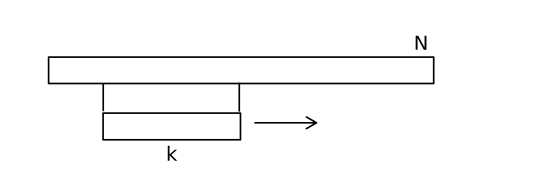
\includegraphics[width=10cm,height=3cm,keepaspectratio]{./Pictures/schiebeArray.png}\\
    \end{itemize}
    \item Suchwort der Länge k $\Rightarrow$ berechne gleitenden Hash für alle Abschnitte der Länge k des Text und vergleiche mit dem Hash des Suchworts
\end{itemize}
\begin{minted}{python}
def rabin_karp_hash(u):
    h = 0
    d,q = 32, 33554393
    for i in u:
        h = (d * h + i) % q
    return h
\end{minted}

\begin{minted}{python}
def rabin_karp_update(c1, c2, k):
    h = (d * h + c2) % q          #rechts ein neues Element hinzufuegen
    h = (h - d ** k * c1) % q   #links eins entfernen
    return h
\end{minted}
